
\documentclass[a4paper,12pt]{article}
\usepackage{enumitem}
\usepackage{graphicx}

\graphicspath{{./assets}}

\title{Arduino-Øving 2\\ \large{IELET1002 Datateknikk}}
\author{Sigmund Klåpbakken}

\begin{document}
\maketitle
\begin{enumerate}
    \item {
    \begin{enumerate}[label=\alph*)]
        \item {A og B er blitt kombinert}
        \item {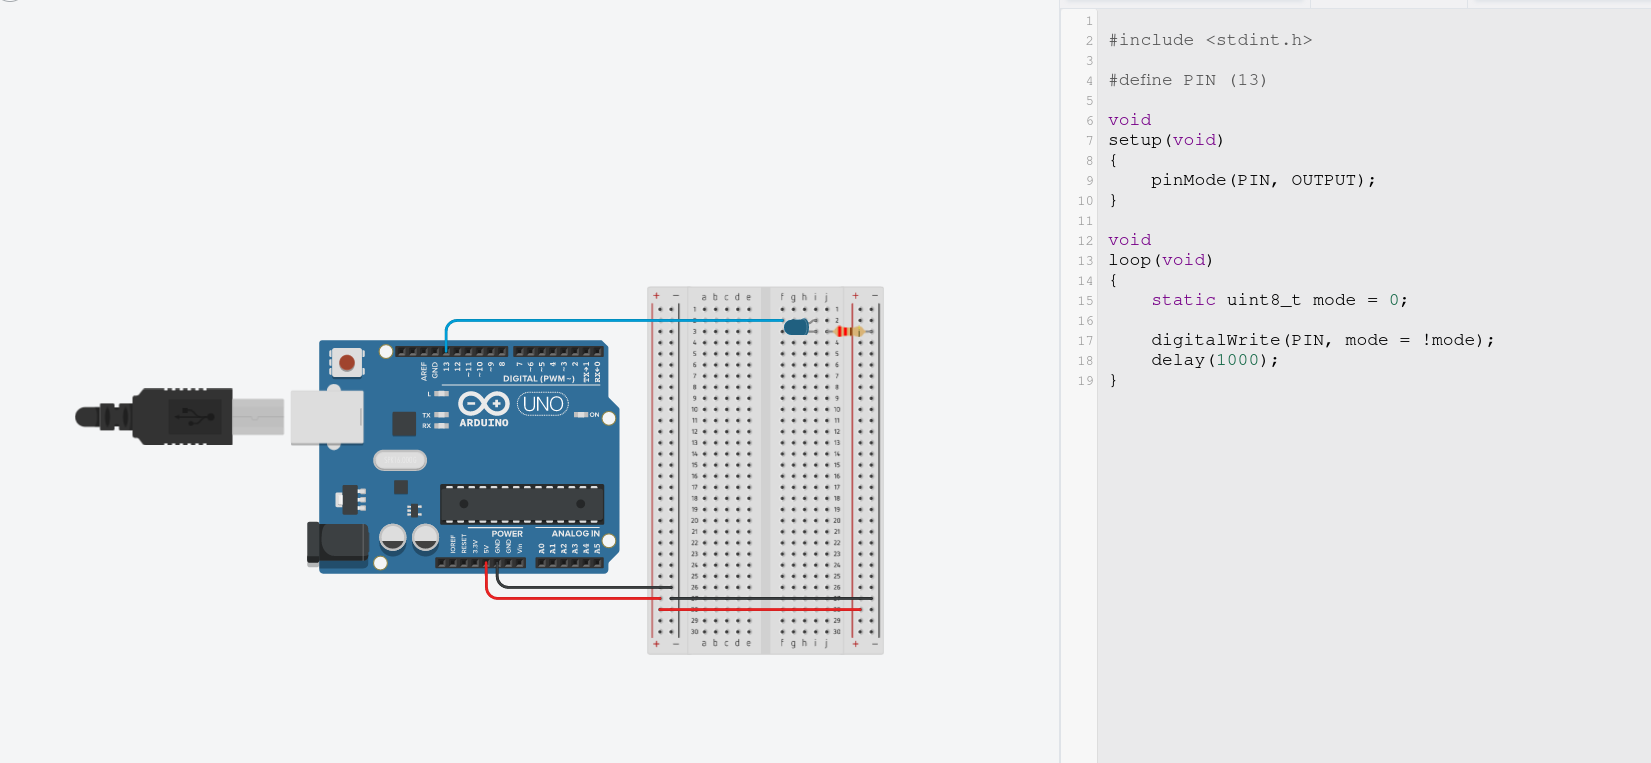
\includegraphics[width=\textwidth]{flash}}
        \item {C og D er blitt kombinert}
        \item {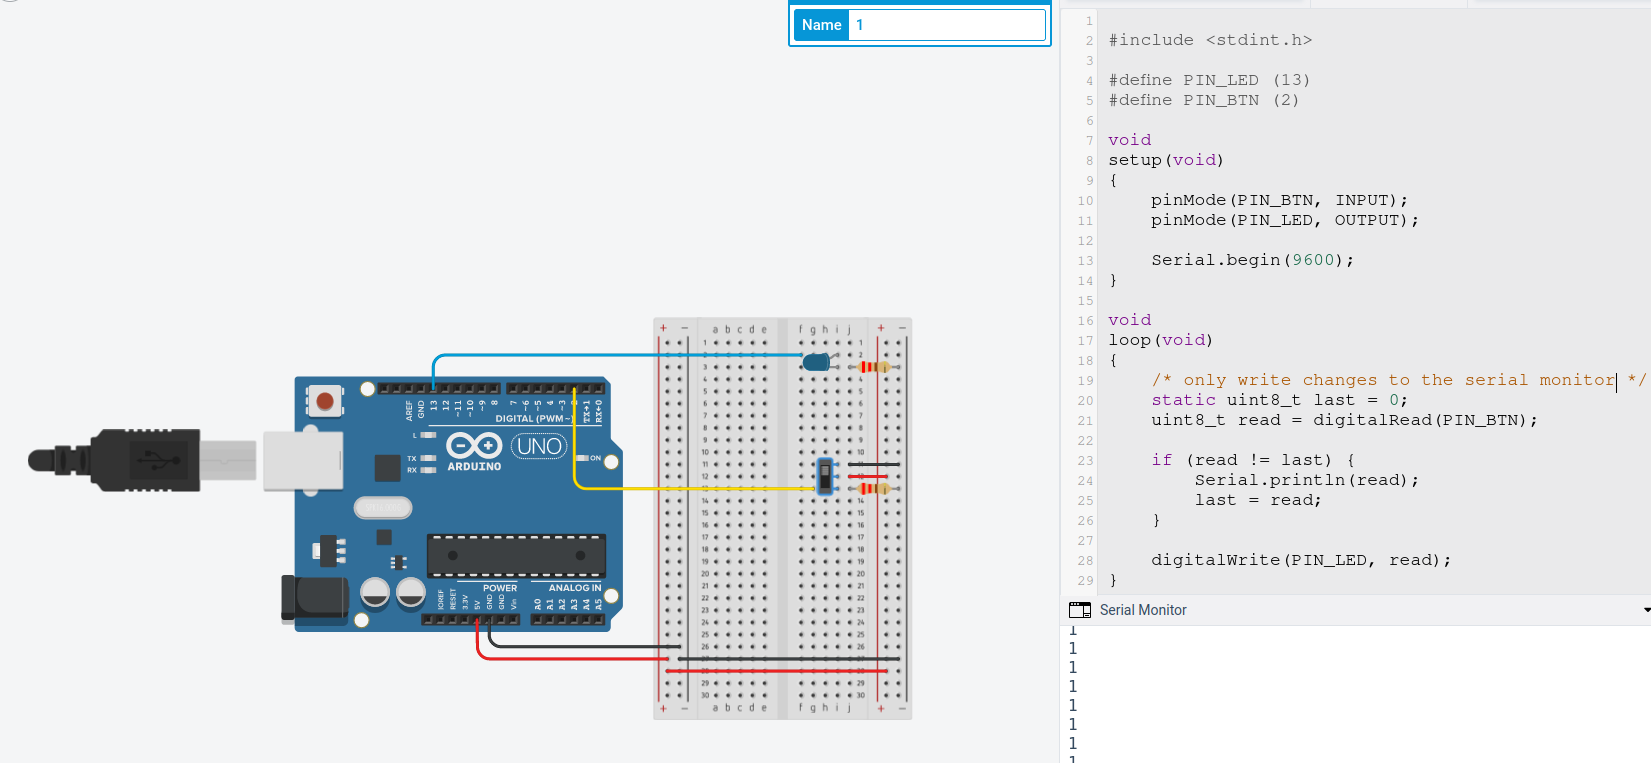
\includegraphics[width=\textwidth]{digitalswitch}}
        \item {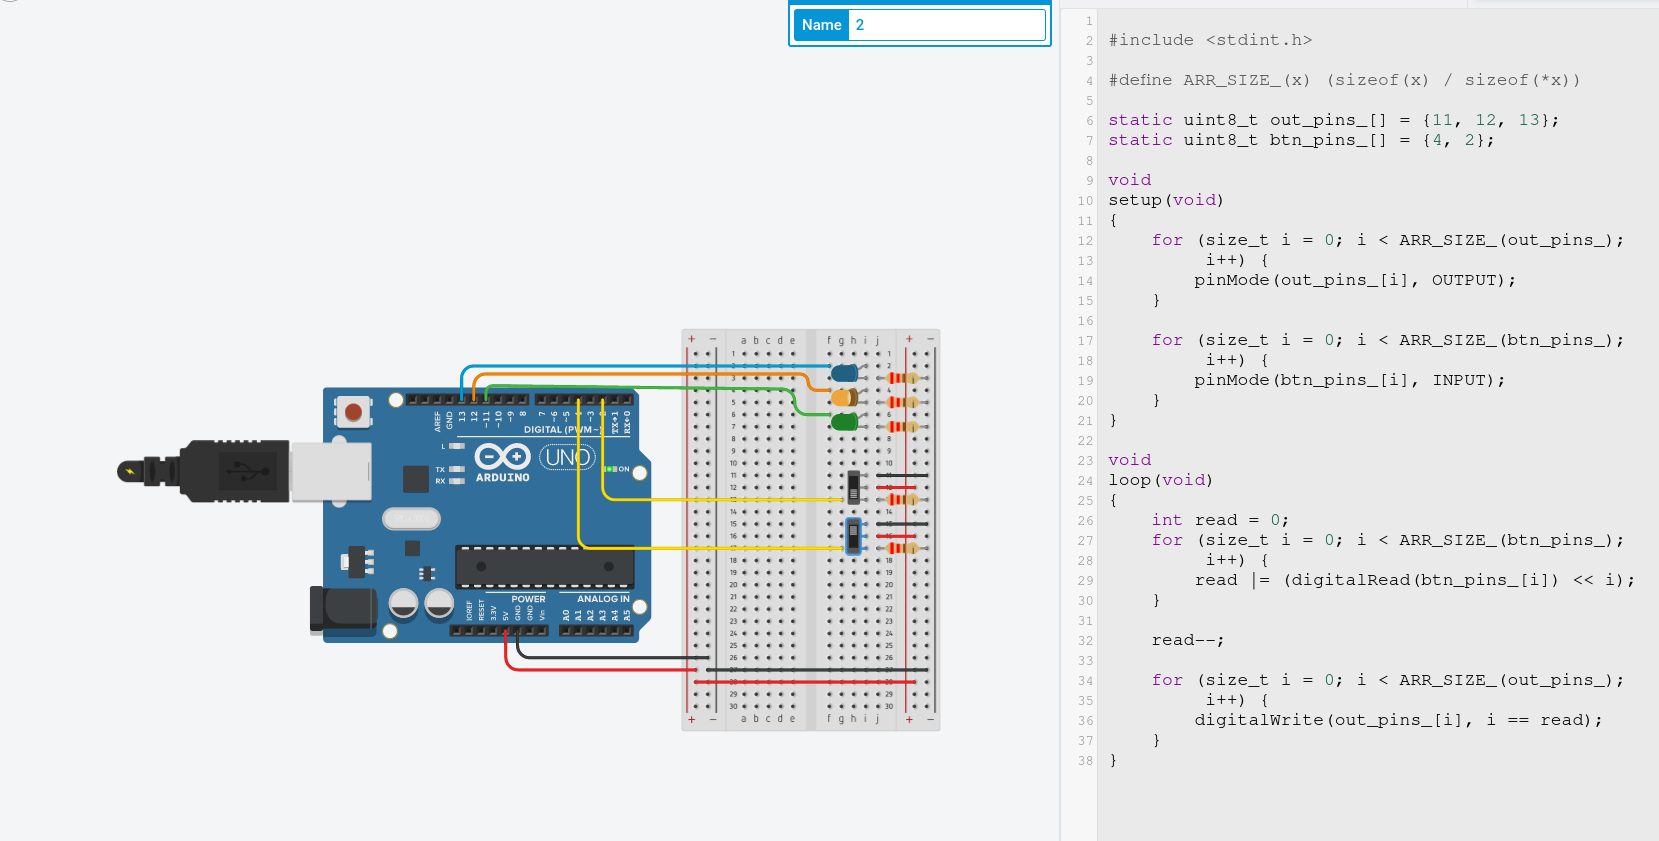
\includegraphics[width=\textwidth]{digitalbin}}
    \end{enumerate}
    \item {
    \begin{enumerate}[label=\alph*)]
        \item {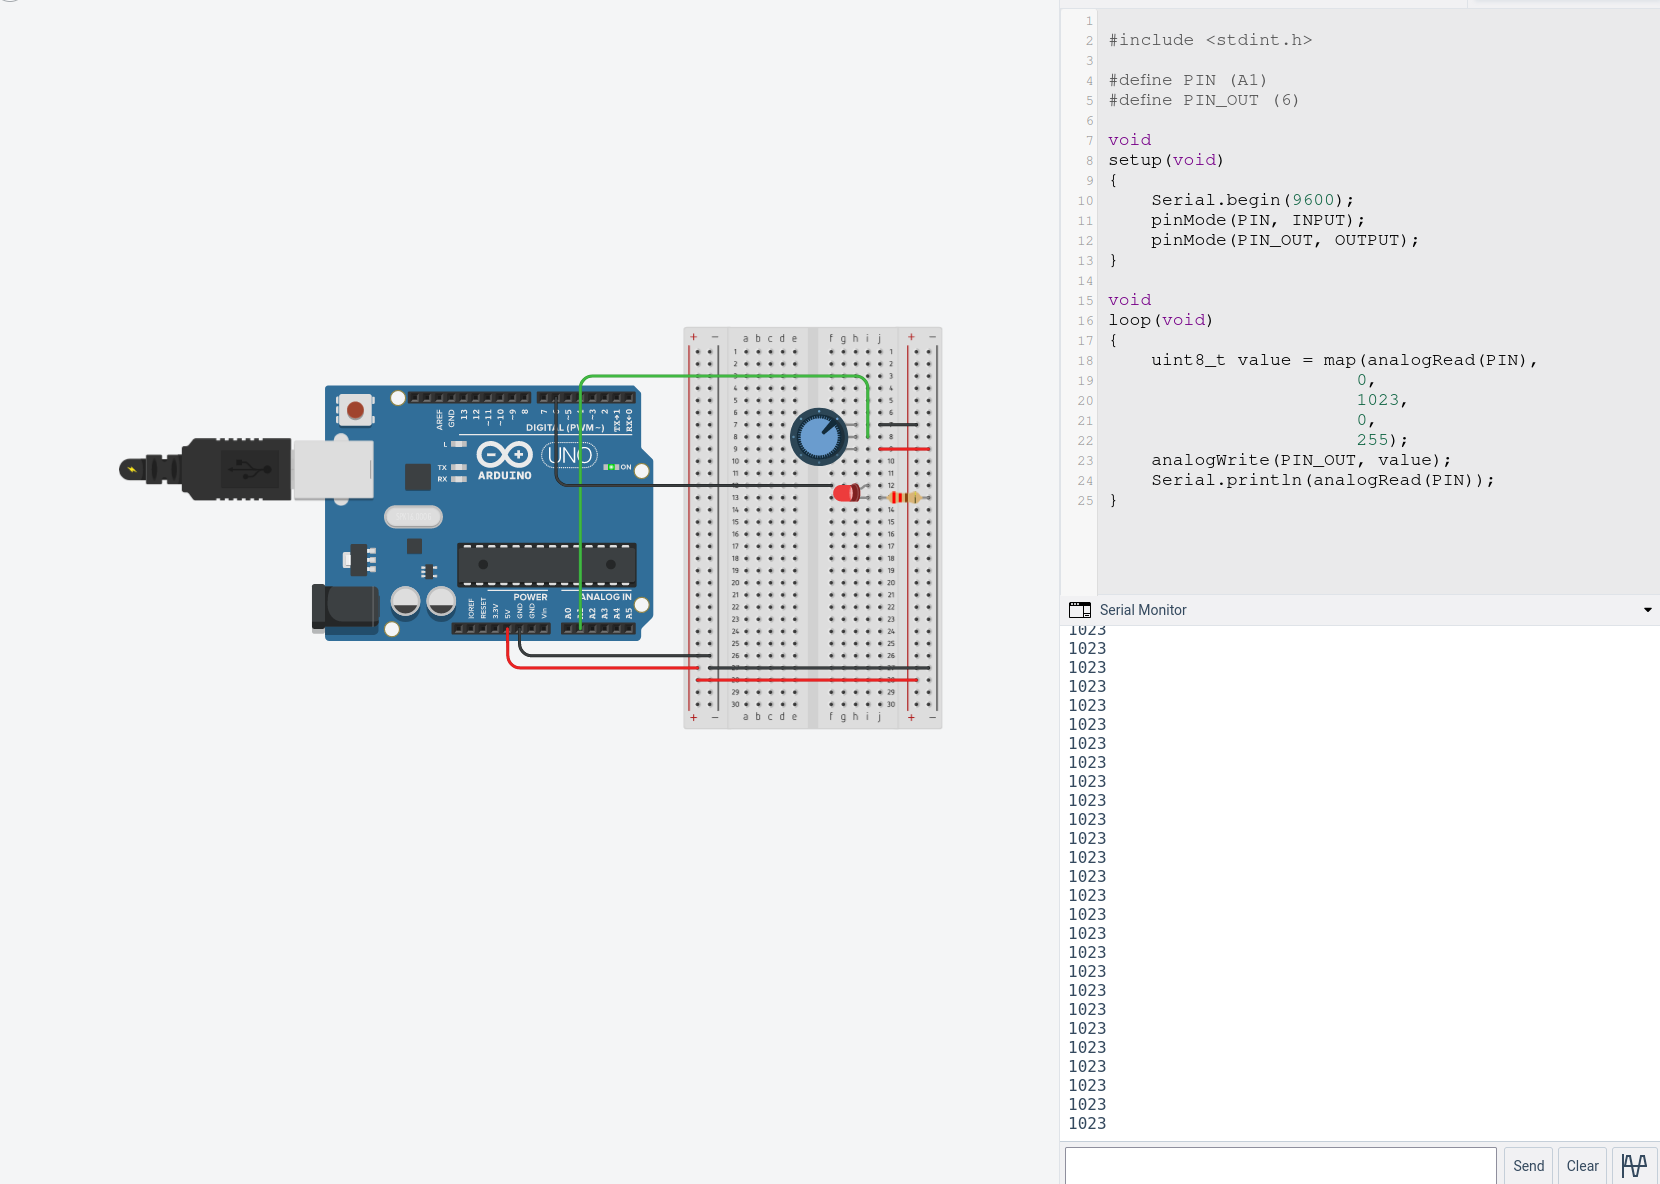
\includegraphics[width=\textwidth]{analog1}}
        \item {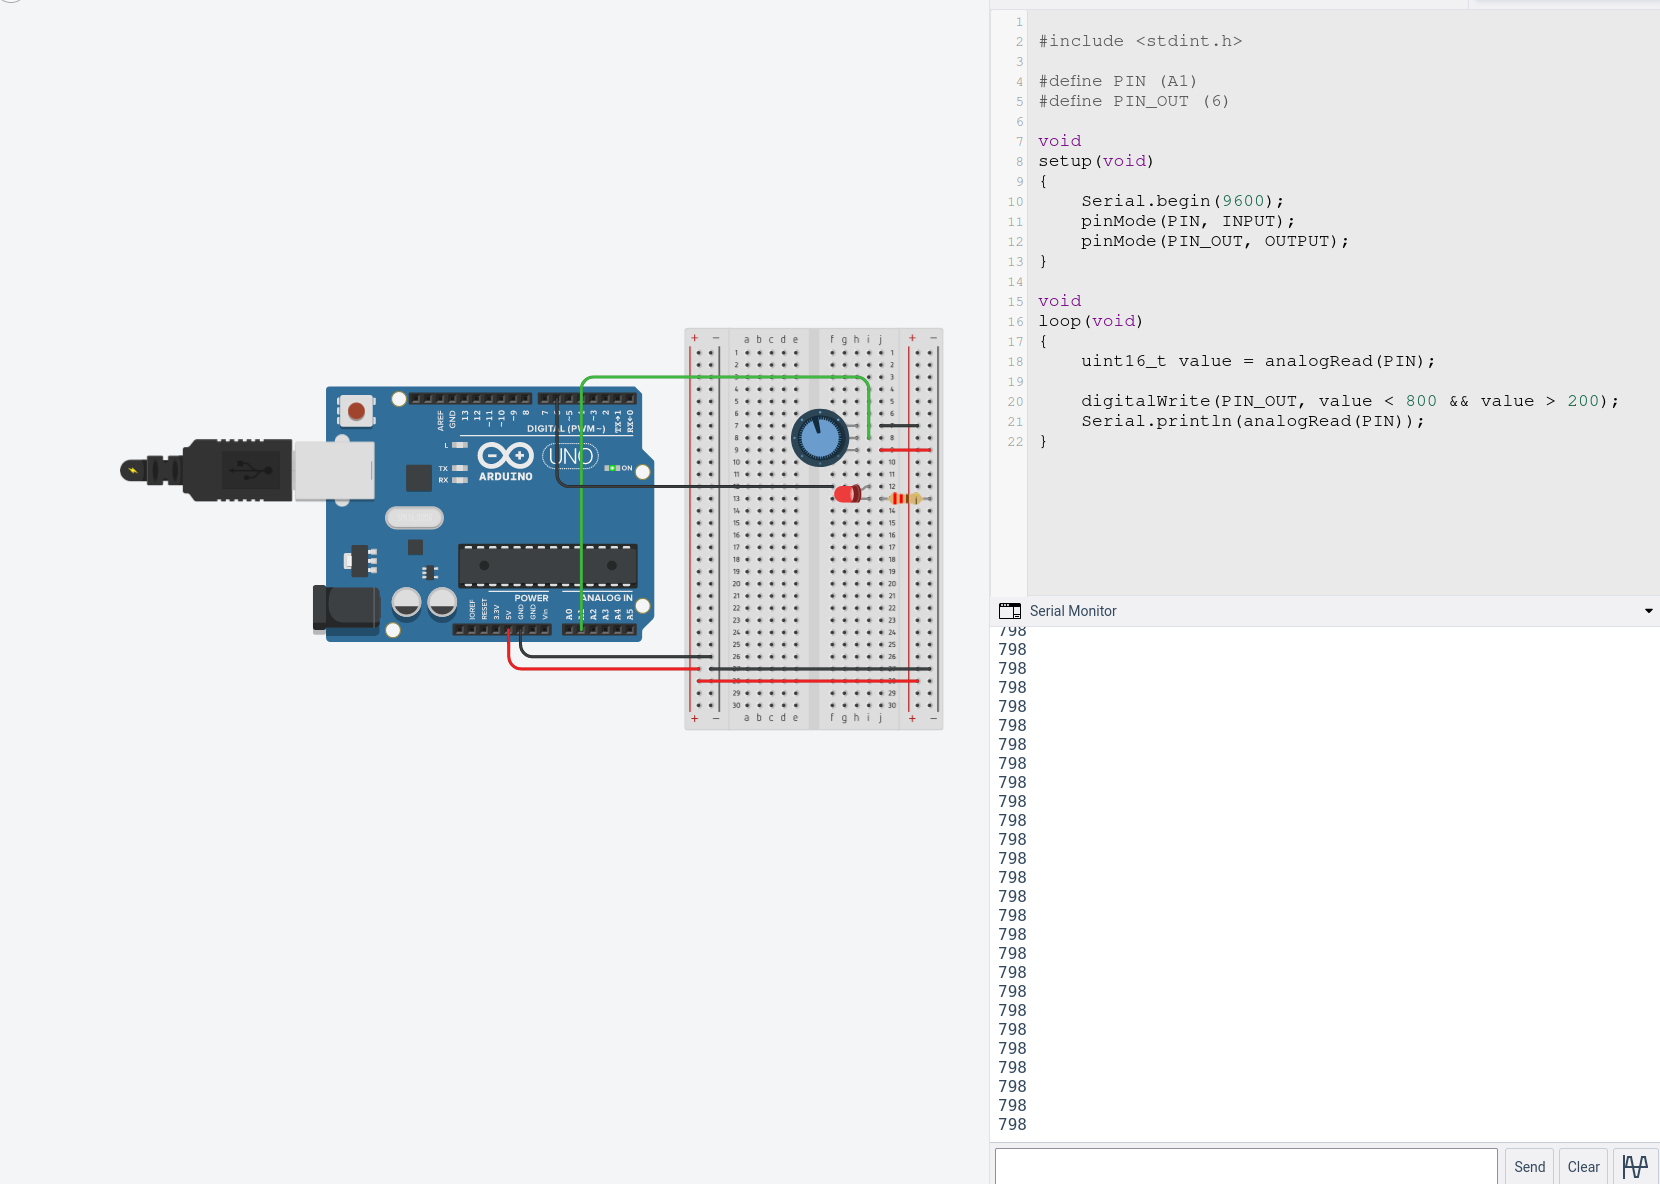
\includegraphics[width=\textwidth]{analog2}}
    \end{enumerate}
    }
    }
\end{enumerate}
\end{document}